\documentclass[compress]{beamer}
\usecolortheme{default}

\usepackage{lmodern, epstopdf, multirow, array, setspace, bbm, tcolorbox, pbox, bm, mathtools, tikz}
\usepackage[T1]{fontenc}

\setbeamertemplate{frametitle}[default][center]
\setbeamertemplate{footline}{\hfill \insertframenumber/\inserttotalframenumber\hspace*{5pt}\vspace{5pt}}
\setbeamertemplate{navigation symbols}{}

\newlength{\wideitemsep}
\setlength{\wideitemsep}{\itemsep}
\addtolength{\wideitemsep}{4pt}
\let\olditem\item
\renewcommand{\item}{\setlength{\itemsep}{\wideitemsep}\olditem}
\setlength{\leftmargini}{12pt}
\setlength{\leftmarginii}{14pt}
\setbeamertemplate{itemize/enumerate subbody begin}{\vspace{6pt}}
\setbeamertemplate{itemize item}[circle]
\setbeamertemplate{enumerate item}[circle]
\setbeamertemplate{enumerate subitem}[default]

\setbeamercolor{alerted text}{fg=blue}
\setbeamersize{text margin left=1.5em,text margin right=1.5em}

\tcbset{
    colback=white,
    colframe=black,
    coltext=black,
    coltitle=blue,
    colbacktitle=white,
    boxrule=1pt,
    titlerule=0pt,
    toptitle=4pt,
    top=2pt
}

\newenvironment{changemargin}[2]{% 
  \begin{list}{}{% 
    \setlength{\topsep}{0pt}% 
    \setlength{\leftmargin}{#1}% 
    \setlength{\rightmargin}{#2}% 
    \setlength{\listparindent}{\parindent}% 
    \setlength{\itemindent}{\parindent}% 
    \setlength{\parsep}{\parskip}% 
  }% 
  \item[]}{\end{list}}
  
\newenvironment{defn}{%
  \begin{tcolorbox}[title={Definition}]%
  }{\end{tcolorbox}}
  
\newenvironment{prop}[1]{%
  \begin{tcolorbox}[title={Proposition #1}]%
  }{\end{tcolorbox}}
  
\newcommand{\cit}[1]{{\footnotesize \textcolor[rgb]{0.5,0,0}{#1}}}

% Font size for code listings (verbatim blocks); reset with \normalsize
\newcommand{\codesize}{\fontsize{7}{8.5}\selectfont}

\newcommand{\slidesetup}[1]{%
  \title{#1}%
  \subtitle{\texorpdfstring{\vspace{0.3\baselineskip}}{} {\small This version: \today}}%
  \author[Mikkel Plagborg-Moller]{ECMA 31150, Spring 2026 \texorpdfstring{\\[0.5ex]}{} University of Chicago \texorpdfstring{\\[0.5ex]}{} Department of Economics \texorpdfstring{\\[4ex]}{} Mikkel Plagborg-Moller}%
  \date{}%
}

% \circleoverlay[options]{text}
% Draws a red circle with a text box nearby on a tikz overlay.
% Options (with defaults):
%   cx=0cm, cy=0cm      - circle center (shift from page center)
%   r=1cm               - circle radius
%   tx=0cm, ty=0cm      - text box offset from circle center
%   text anchor=east    - anchor of text node (east = text left, west = text right)
%   font=\normalsize    - font size for text
\pgfkeys{
  /circleoverlay/.cd,
  cx/.store in=\cocx, cx=0cm,
  cy/.store in=\cocy, cy=0cm,
  r/.store in=\cor, r=1cm,
  tx/.store in=\cotx, tx=0cm,
  ty/.store in=\coty, ty=0cm,
  text anchor/.store in=\cotextanchor, text anchor=east,
  font/.store in=\cofont, font=\normalsize,
}
\newcommand{\circleoverlay}[2][]{%
  \pgfkeys{/circleoverlay/.cd, cx=0cm, cy=0cm, r=1cm, tx=0cm, ty=0cm, text anchor=east, font=\normalsize, #1}%
  \pgfmathsetlengthmacro{\circlediameter}{2*\cor}%
  \node[draw=red, line width=2pt, circle, minimum size=\circlediameter, inner sep=0pt]
    (tmpcirc) at ([xshift=\cocx,yshift=\cocy]current page.center) {};%
  \node[anchor=\cotextanchor, fill=white, draw=red, text=red, inner sep=4pt, align=left, font=\cofont]
    at ([xshift=\cotx,yshift=\coty]tmpcirc.center) {#2};%
}

\DeclareMathOperator*{\argmax}{argmax}
\DeclareMathOperator*{\argmin}{argmin}
\DeclareMathOperator{\diag}{diag}
\DeclareMathOperator{\var}{Var}
\DeclareMathOperator{\cov}{Cov}
\DeclareMathOperator{\corr}{Corr}
\DeclareMathOperator{\lrv}{LRV}


\slidesetup{Vector autoregression II}

\begin{document}
\frame{
\maketitle
}

\frame{
\frametitle{Plan for this slide deck}
\begin{enumerate}
\item How to convert a VAR($p$) model to VAR(1) so we can\dots
\begin{itemize}
\item Check stationarity
\item Forecast
\item Compute moments
\end{itemize}
\item VARMA model, matrix lag polynomials
\item VAR bootstrap for more accurate small-sample inference
\end{enumerate}
}

\frame{
\frametitle{VAR($p$): companion form}
\[\bm{y}_t = \bm{c} + \bm{A}_1\bm{y}_{t-1} + \dots + \bm{A}_p\bm{y}_{t-p} + \bm{u}_t\]
\begin{itemize}
\item When is the model cov.\ stationary? How do we forecast? What are the moments?
\item Everything will follow from our previous VAR(1) results after we perform a neat trick\dots
\end{itemize}
}

\frame{
\frametitle{VAR($p$): companion form (cont.)}
\begin{itemize}
\item \alert{Claim:} the VAR($p$) model with $n$ variables is \emph{equivalent} with the following \textbf{companion form} VAR(1) model with $n \times p$ variables:
\[\tilde{\bm{y}}_t = \tilde{\bm{c}} + \tilde{\bm{A}}\tilde{\bm{y}}_{t-1} + \tilde{\bm{u}}_t,\quad \text{where}\]

\[\tilde{\bm{y}}_t \equiv \underbrace{\begin{pmatrix}
\bm{y}_t \\
\bm{y}_{t-1} \\
\vdots \\
\bm{y}_{t-p+1}
\end{pmatrix}}_{np \times 1},\quad \tilde{\bm{c}} \equiv \underbrace{\begin{pmatrix}
\bm{c} \\
\bm{0} \\
\vdots \\
\bm{0}
\end{pmatrix}}_{np \times 1},\quad \tilde{\bm{u}}_t \equiv \underbrace{\begin{pmatrix}
\bm{u}_t \\
\bm{0} \\
\vdots \\
\bm{0}
\end{pmatrix}}_{np \times 1},\]
\[\tilde{\bm{A}} \equiv \underbrace{\left(\begin{array}{ccc|c}
\bm{A}_1 & \cdots & \bm{A}_{p-1} & \bm{A}_p \\
\hline
\multicolumn{3}{c|}{\bm{I}_{n(p-1)}} & \bm{0}_{n(p-1) \times n}
\end{array}\right)}_{np \times np}.\]
\end{itemize}
}

\frame{
\frametitle{VAR($p$): companion form (cont.)}
\begin{itemize}
\item Example: consider a univariate AR(2) model
\[y_t = c + a_1 y_{t-1} + a_2 y_{t-2} + u_t.\]
\item Companion form:
\[\begin{pmatrix}
y_t \\
y_{t-1}
\end{pmatrix} = \begin{pmatrix}
c \\
0
\end{pmatrix} + \begin{pmatrix}
a_1 & a_2 \\
1 & 0
\end{pmatrix} \begin{pmatrix}
y_{t-1} \\
y_{t-2}
\end{pmatrix} + \begin{pmatrix}
u_t \\
0
\end{pmatrix}.\]
Only the first equation is non-vacuous.
\item \alert{Exercise:} do the same for an AR(3) model.
\end{itemize}
}

\frame{
\frametitle{VAR($p$): companion form (cont.)}
\begin{itemize}
\item When does a VAR($p$) model have a cov.\ stationary solution?
\begin{itemize}
\item Answer: when the companion form VAR matrix $\tilde{\bm{A}}$ has all its eigenvalues inside the unit circle.
\end{itemize}
\item How can we forecast (one-step or multi-step) with a VAR($p$) model?
\begin{itemize}
\item Answer: rewrite model in companion form, then apply the simple VAR(1) formulas.
\end{itemize}
\item What are the moments of the variables in a VAR($p$) model?
\begin{itemize}
\item Answer: write model in companion form and use the VAR(1) formulas.
\end{itemize}
\end{itemize}
}

\frame{
\frametitle{VARMA models}
\begin{itemize}
\item Vector ARMA (\textbf{VARMA}) model:
\[\bm{y}_t = \bm{c} + \bm{A}_1\bm{y}_{t-1} + \dots + \bm{A}_p\bm{y}_{t-p} + \bm{u}_t + \bm{\Theta}_1 \bm{u}_{t-1} + \dots + \bm{\Theta}_q \bm{u}_{t-q},\]
where $\bm{\Theta}_1,\dots,\bm{\Theta}_q$ are $n \times n$ matrices.
\item Can write this with \textbf{matrix lag polynomial} notation:
\[\bm{A}(L)\bm{y}_t = \bm{c} + \bm{\Theta}(L)\bm{u}_t, \quad \text{where}\]
\[\bm{A}(L) \equiv \bm{I} - \sum_{\ell=1}^p \bm{A}_\ell L^\ell,\quad \bm{\Theta}(L) \equiv \bm{I} + \sum_{\ell=1}^q \bm{\Theta}_\ell L^\ell.\]
\item Matrix lag polynomials work like scalar ones, except they don't necessarily commute (like ordinary matrices): $\bm{B}(L)\bm{C}(L) \neq \bm{C}(L)\bm{B}(L)$.
\end{itemize}
}

\frame{
\frametitle{Finite-sample properties of VAR estimator}
\begin{itemize}
\item The OLS estimator for VAR($p$) models is approximately unbiased and normally distributed when the sample size $T$ is large.
\item But as we saw for AR models, when $T$ is small/moderate and the data is very persistent, the estimator could be quite biased and non-normally distributed.
\item As a result, the standard OLS confidence intervals may not have coverage probability close to the nominal level.
\end{itemize}
}

\frame{
\frametitle{Bootstrap}
\begin{itemize}
\item The \textbf{bootstrap} is a method for obtaining a better approximation to the small-sample distribution of the VAR estimator than that provided by asymptotic theory.
\item Instead of theoretical approximations, the bootstrap leverages computing power.
\item The basic idea is to \textbf{resample} the data many times:
\begin{itemize}
\item Generate 100s of simulated data sets that mimic the actual data generating process.
\item Compute the VAR estimator on each of the simulated data sets.
\item This traces out a sampling distribution for the VAR estimator across \emph{simulated} data sets.
\item Hopefully provides a good approximation to the sampling distribution across \emph{hypothetical histories of the real world}.
\end{itemize}
\end{itemize}
}

\frame{
\frametitle{Bootstrap: motivation}
\begin{itemize}
\item Consider a VAR(1) model with i.i.d.\ innovations:
\[\bm{y}_t = \bm{c} + \bm{A}\bm{y}_{t-1} + \bm{u}_t,\quad \bm{u}_t \overset{iid}{\sim} (\bm{0},\bm{\Sigma}).\]
\vspace{-1.5\baselineskip}
\begin{itemize}
\item Could be companion form of a VAR($p$) model.
\end{itemize}
\item We want to understand the bias and distributional properties of the OLS estimator $\hat{\bm{A}}$ in a given sample size $T$.
\item Suppose for a moment that we \emph{knew} the true VAR coefficients $\bm{c},\bm{A}$ and the true distribution of $\bm{u}_t$ (a bit silly, but stay with me!).
\item Then the most straight-forward way to find the distribution of $\hat{\bm{A}}$ is through \textbf{Monte Carlo simulation} (we already did this in an earlier slide deck).
\end{itemize}
}

\frame{
\frametitle{Monte Carlo simulation: algorithm}
\begin{enumerate}
\item Choose a large $B$ (e.g., 1000).
\item In each \textbf{iteration} $b=1,2,\dots,B$:
\begin{enumerate}[a)]
\item Simulate shocks $\bm{u}_2^*,\dots,\bm{u}_T^*$ from the \alert{known} distribution of $\lbrace \bm{u}_t \rbrace$.
\item Generate a fake data set $\lbrace \bm{y}_t^* \rbrace_{t=1}^T$ satisfying the \alert{known} model:
\[\bm{y}_t^* = \bm{c} + \bm{A} \bm{y}_{t-1}^* + \bm{u}_t^*,\quad t=2,\dots,T,\]
given an initial value $\bm{y}_1^*$ drawn from a \alert{known} distribution.
\item Compute the VAR OLS estimator $\hat{\bm{A}}_{(b)}^*$ on the fake sample $\lbrace \bm{y}_1^*,\dots,\bm{y}_T^* \rbrace$.
\end{enumerate}
\item The histogram of the $B$ simulated estimates $\hat{\bm{A}}_{(1)}^*,\dots,\hat{\bm{A}}_{(B)}^*$ approximates the actual sampling distribution of the VAR OLS estimator for sample size $T$.
\end{enumerate}
}

\frame{
\begin{figure}
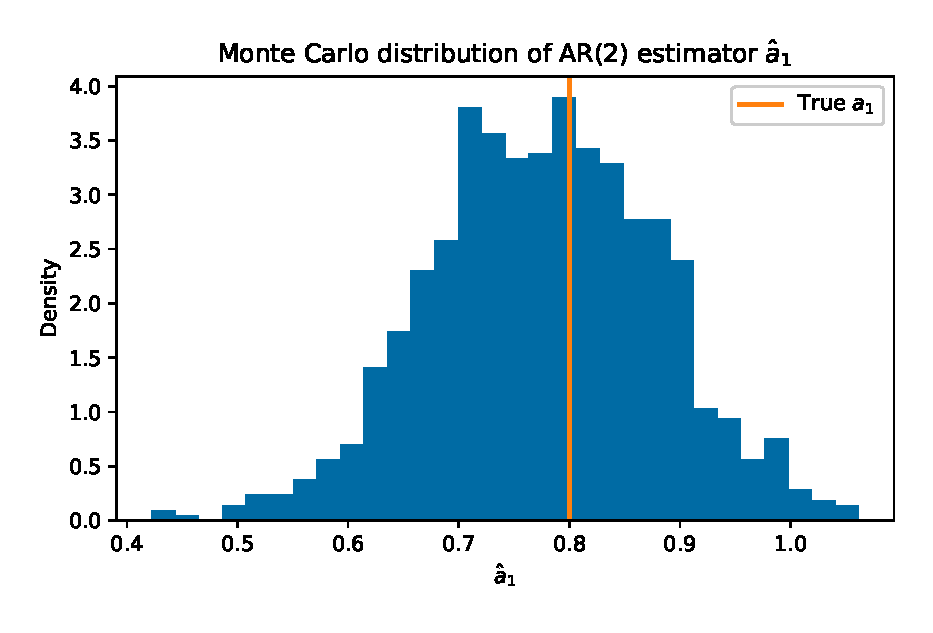
\includegraphics[width=\linewidth]{fig/ar2_mc_hist.eps} \\
\vspace{-1.5\baselineskip}
\[y_t = c + a_1 y_{t-1} + a_2 y_{t-2} + u_t, \quad u_t \overset{iid}{\sim} N(0,\sigma^2),\]
\[c=0,\; a_1=0.8,\; a_2=0.1,\; \sigma^2=1,\quad T=100,\quad B=1000\]
\end{figure}
}

\frame{
\frametitle{Recursive residual bootstrap}
\begin{itemize}
\item The preceding strategy is infeasible in practice, since we know neither the model coefficients, nor the shock distribution.
\item But we can \emph{estimate} these:
\begin{itemize}
\item Approximate the true $\bm{c},\bm{A}$ with the real-data estimates $\hat{\bm{c}},\hat{\bm{A}}$.
\item Approximate the shock distribution by the empirical distribution of the OLS residuals $\hat{\bm{u}}_2,\dots,\hat{\bm{u}}_T$.
\end{itemize}
\item Plugging these estimates of the true parameters into the previous Monte Carlo recipe yields the \textbf{recursive residual bootstrap}.
\end{itemize}
}

\frame{
\frametitle{Recursive residual bootstrap: algorithm}
\begin{enumerate}
\item Compute real-data OLS estimates $\hat{\bm{c}},\hat{\bm{A}}$ and residuals $\hat{\bm{u}}_2,\dots,\hat{\bm{u}}_T$.
\item Choose a large $B$ (e.g., 1000).
\item In each iteration $b=1,2,\dots,B$:
\begin{enumerate}[a)]
\item Draw $T-1$ shock vectors $\bm{u}_2^*,\dots,\bm{u}_T^*$ uniformly at random (with replacement) from the list $\alert{\hat{\bm{u}}_2,\dots,\hat{\bm{u}}_T}$.
\item Generate a fake data set $\lbrace \bm{y}_t^* \rbrace_{t=1}^T$ recursively:
\[\bm{y}_t^* = \alert{\hat{\bm{c}}} + \alert{\hat{\bm{A}}} \bm{y}_{t-1}^* + \bm{u}_t^*,\quad t=2,3,\dots,T,\]
given an initial value $\alert{\bm{y}_1^*}$ (more on next slide).
\item Compute the VAR OLS estimator $\hat{\bm{A}}_{(b)}^*$ on the fake sample $\lbrace \bm{y}_1^*,\dots,\bm{y}_T^* \rbrace$.
\end{enumerate}
\item The histogram of the $B$ bootstrap estimates $\hat{\bm{A}}_{(1)}^*,\dots,\hat{\bm{A}}_{(B)}^*$ approximates the sampling distribution of $\hat{\bm{A}}$ in the real data.
\end{enumerate}
}

\frame{
\frametitle{Recursive residual bootstrap: initial values}
\begin{itemize}
\item When simulating bootstrap data $\lbrace \bm{y}_t^* \rbrace$, we need to pick an initial value $\bm{y}_1^*$.
\item It's customary to pick this value uniformly at random from the real data set, independently in each bootstrap iteration.
\item VAR($p$) generalization: need $p$ initial values. We can pick $p$ consecutive observations uniformly at random from the real data as initial values.
\end{itemize}
}

\begin{frame}[fragile]
\frametitle{Recursive residual bootstrap: example}
\begin{itemize}
\item The VAR(1) algorithm easily generalizes to VAR($p$).
\item Let's do an AR(2) example for concreteness.
\end{itemize}
\bigskip

\footnotesize
\begin{verbatim}
# Load data
df = pd.read_csv('data/CPIAUCSL.csv', index_col='observation_date',
    parse_dates=True)
df = df.interpolate() # interpolate missing value in Oct 2025
cpi = df['CPIAUCSL'].values
y = 100*np.diff(np.log(cpi)) # monthly inflation rate

# Estimate AR(2) model
result = sm.tsa.AutoReg(y, lags=2).fit()
print(result.summary())
\end{verbatim}
\end{frame}

\begin{frame}[fragile]
\scriptsize
\begin{verbatim}
                            AutoReg Model Results                             
==============================================================================
Dep. Variable:                      y   No. Observations:                  949
Model:                     AutoReg(2)   Log Likelihood                -113.499
Method:               Conditional MLE   S.D. of innovations              0.273
Date:                Wed, 08 Apr 2026   AIC                            234.999
Time:                        09:11:22   BIC                            254.412
Sample:                             2   HQIC                           242.397
                                  949                                         
==============================================================================
                 coef    std err          z      P>|z|      [0.025      0.975]
------------------------------------------------------------------------------
const          0.1081      0.012      8.823      0.000       0.084       0.132
y.L1           0.5047      0.032     15.802      0.000       0.442       0.567
y.L2           0.1126      0.032      3.529      0.000       0.050       0.175
\end{verbatim}
\end{frame}

\begin{frame}[fragile]
\footnotesize
\begin{verbatim}
param_hat = result.params
u_hat = result.resid # residuals (length T-2)
T = len(y)

B = 1000 # number of bootstrap samples

param_hat_boot = np.empty((B, 3))
for b in range(B):
    # Resample residuals with replacement
    u_boot = rng.choice(u_hat, size=T - 2, replace=True)
    # Initial values: random pair of consecutive obs.
    i0 = rng.integers(0, T - 1)
    y_init = y[i0:i0 + 2]
    # Simulate bootstrap sample and estimate
    y_boot = simulate_ar2(param_hat, u_boot, y_init)
    result_boot = sm.tsa.AutoReg(y_boot, lags=2).fit()
    param_hat_boot[b] = result_boot.params
\end{verbatim}
\bigskip
\normalsize Note: the \texttt{simulate\_ar2} function is defined by me (not shown here).
\end{frame}

\frame{
\begin{figure}
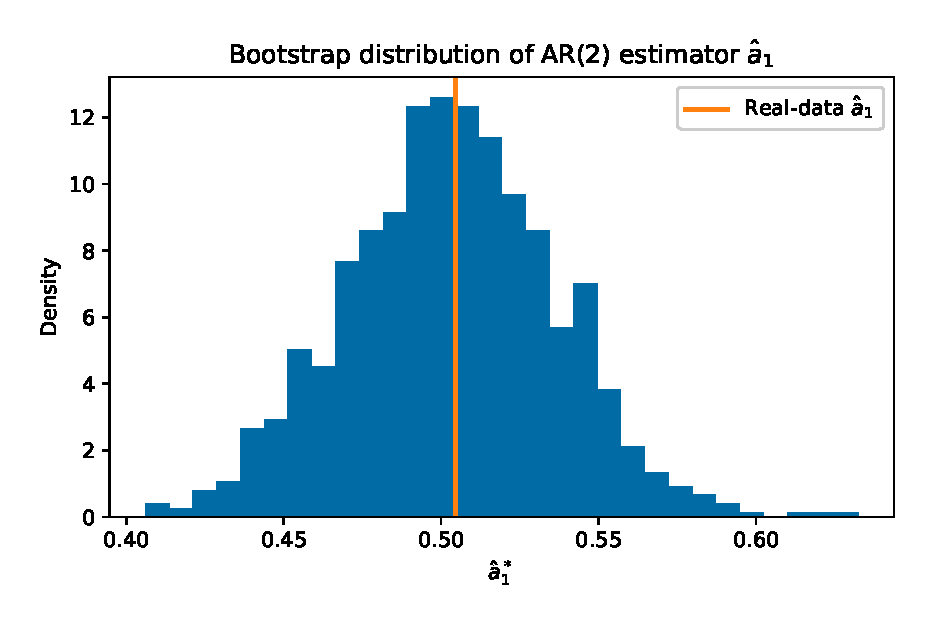
\includegraphics[width=\linewidth]{fig/ar2_boot_hist.eps}
\end{figure}
}

\frame{
\frametitle{Bootstrap approximation of sampling distribution}
\begin{itemize}
\item The coefficients that generate the bootstrap data sets are $\hat{\bm{A}}$.
\item Hence, the distribution of $\hat{\bm{A}}^*-\hat{\bm{A}}$ across bootstrap iterations is analogous to the distribution of $\hat{\bm{A}}-\bm{A}$ across (hypothetical) repeated samples of the real data.
\begin{itemize}
\item $\bm{A}$: true coefficients that generated the real data.
\end{itemize}
\item \alert{Result:} the bootstrap distribution of $\hat{\bm{A}}^*-\hat{\bm{A}}$ approximates the sampling distribution of $\hat{\bm{A}}-\bm{A}$ arbitrarily well as $T \to \infty$.
\begin{itemize}
\item Assumes the data follows a stationary VAR(1) model with i.i.d.\ shocks.
\end{itemize}
\item In practice for small/moderate $T$, the bootstrap approximation is typically more accurate than the approximation provided by our usual analytical asymptotic formulas (used in regression software).
\end{itemize}
}


\begin{frame}[fragile]
\frametitle{Bootstrap standard errors}
\begin{itemize}
\item We would like to report standard errors (SEs) for our VAR estimator. SE = estimate of the standard deviation of an element $\hat{A}_{ij}$ of the matrix $\hat{\bm{A}}$.
\item We can use the bootstrap distribution to compute SEs.
\item The \textbf{bootstrap standard error} of the estimator $\hat{A}_{ij}$ is the sample standard deviation of $\hat{A}_{ij}^*$ across the $B$ bootstrap draws.
\end{itemize}
\bigskip
\begin{verbatim}
# Bootstrap SE
se_boot = np.std(param_hat_boot, axis=0, ddof=1)
\end{verbatim}
\end{frame}

\frame{
\frametitle{Bootstrap confidence interval}
\begin{itemize}
\item We want a confidence interval (CI) for $A_{ij}$.
\item Let $\tilde{q}_\alpha$ be the $\alpha$-quantile of the sampling distribution of $\hat{A}_{ij}-A_{ij}$ in the real data. By definition,
\[P\left(\tilde{q}_{\alpha/2} \leq \hat{A}_{ij}-A_{ij} \leq \tilde{q}_{1-\alpha/2} \right) = 1-\alpha.\]
\item Let $\tilde{q}_\alpha^*$ be the $\alpha$-quantile of $\hat{A}_{ij}^*-\hat{A}_{ij}$ across the $B$ bootstrap draws (i.e., the $(\alpha \times B)$-th smallest value).
\item Because the bootstrap distribution of $\hat{A}_{ij}^*-\hat{A}_{ij}$ approximates the sampling distribution of $\hat{A}_{ij}-A_{ij}$,
\[\tilde{q}_\alpha^* \approx \tilde{q}_\alpha\quad \text{for all }\alpha\]
\[\Longrightarrow\quad P\left(\tilde{q}_{\alpha/2}^* \leq \hat{A}_{ij}-A_{ij} \leq \tilde{q}_{1-\alpha/2}^* \right) \approx 1-\alpha.\]
\end{itemize}
}

\frame{
\frametitle{Bootstrap confidence interval (cont.)}
\[P\left(\tilde{q}_{\alpha/2}^* \leq \hat{A}_{ij}-A_{ij} \leq \tilde{q}_{1-\alpha/2}^* \right) \approx 1-\alpha\]
\vspace{-0.5\baselineskip}
\begin{itemize}
\item Rearrange the inequalities:
\[P\left(\hat{A}_{ij}-\tilde{q}_{1-\alpha/2}^* \leq A_{ij} \leq \hat{A}_{ij} - \tilde{q}_{\alpha/2}^*\right) \approx 1-\alpha.\]
\item \alert{Conclusion:} the \textbf{bootstrap confidence interval}
\[\hat{\mathcal{I}}^* \equiv \left[\hat{A}_{ij}-\tilde{q}_{1-\alpha/2}^*, \hat{A}_{ij} - \tilde{q}_{\alpha/2}^*\right]\]
has approximately correct coverage:
\[\boxed{P\left(A_{ij} \in \hat{\mathcal{I}}^*\right) \approx 1-\alpha}.\]
(This becomes an equality in the limit $T \to \infty$.)
\end{itemize}
}

\begin{frame}[fragile]
\frametitle{Bootstrap confidence interval: alternative formula}
\begin{itemize}
\item Since $\hat{A}_{ij}$ doesn't change across bootstrap iterations (only $\hat{A}_{ij}^*$ does),
\[\tilde{q}_\alpha^* = q_\alpha^* - \hat{A}_{ij},\]
where $q_\alpha^*$ is the $\alpha$-th sample quantile of $\hat{A}_{ij}^*$ across bootstrap draws.
\item Hence, we can equivalently write the bootstrap CI as
\[\hat{\mathcal{I}}^* = \left[2\hat{A}_{ij}-q_{1-\alpha/2}^*, 2\hat{A}_{ij} - q_{\alpha/2}^*\right].\]
\vspace{-1.5\baselineskip}
\begin{itemize}
\item Note: the $1-\alpha/2$ quantile appears in the \emph{left} end point of the interval, while the $\alpha/2$ quantile appears in the \emph{right} end point.
\end{itemize}
\end{itemize}
\bigskip
\scriptsize
\begin{verbatim}
# Bootstrap confidence intervals
signif = 0.05
ci_lower = 2*param_hat - np.quantile(param_hat_boot, 1 - signif/2, axis=0)
ci_upper = 2*param_hat - np.quantile(param_hat_boot, signif/2, axis=0)
\end{verbatim}
\end{frame}

\begin{frame}[fragile]
\begin{verbatim}
       Estimate      SE  CI lower  CI upper
const    0.1081  0.0125    0.0810    0.1302
a1       0.5047  0.0331    0.4430    0.5700
a2       0.1126  0.0317    0.0532    0.1811
\end{verbatim}
\bigskip
\begin{itemize}
\item In this case, the bootstrap SEs and CIs are close to the analytical ones shown on an earlier slide.
\item This is because the data is only moderately persistent and $T$ is fairly large.
\item In other data sets, the bootstrap can give very different results from analytical inference.
\end{itemize}
\end{frame}

\frame{
\frametitle{Bootstrap confidence interval: implicit bias correction}
\[\hat{\mathcal{I}}^* = \left[2\hat{A}_{ij}-q_{1-\alpha/2}^*, 2\hat{A}_{ij} - q_{\alpha/2}^*\right]\]
\vspace{-0.5\baselineskip}
\begin{itemize}
\item The bootstrap CI may not be symmetric around $\hat{A}_{ij}$.
\item If the bootstrap draws $\hat{A}_{ij}^*$ tend to be below $\hat{A}_{ij}$ (indicating downward bias), then $\hat{\mathcal{I}}^*$ is centered \emph{above} $\hat{A}_{ij}$ -- implicitly correcting the bias! (Though not perfectly.)
\item Compare with the usual analytical confidence interval:
\[\hat{\mathcal{I}} \equiv \left[\hat{A}_{ij}-\mathit{SE}(\hat{A}_{ij})Q_{1-\alpha/2}, \hat{A}_{ij} + \mathit{SE}(\hat{A}_{ij})Q_{1-\alpha/2}\right],\]
where $Q_{1-\alpha/2}$ is the $(1-\alpha/2)$-quantile of the standard normal distribution. This CI is symmetric around the (biased) estimator $\hat{A}_{ij}$.
\end{itemize}
}

\frame{
\frametitle{Efron's bootstrap confidence interval}
\begin{itemize}
\item Suppose it happened to be the case that the bootstrap distribution of $\hat{A}_{ij}^*$ was exactly symmetric around $\hat{A}_{ij}$. Then
\[q_{1-\alpha/2}^* - \hat{A}_{ij} = \hat{A}_{ij} - q_{\alpha/2}^*.\]
\item Then the bootstrap CI would equal
\[\hat{\mathcal{I}}^* = \left[q_{\alpha/2}^*, q_{1-\alpha/2}^*\right].\]
\item The above CI formula is called the \textbf{Efron bootstrap confidence interval}. It's popular in practice, but typically has less accurate coverage than our earlier CI, unless the estimator is nearly symmetrically distributed around the true parameter.
\end{itemize}
}

\frame{
\frametitle{Bootstrap: extensions}
\begin{enumerate}
\item In my example code, I've worked with an AR(2) model. In the pset, you will work with a more general VAR($p$) model.
\item Suppose we want to do inference on any function $g(\bm{A},\bm{\Sigma})$ of the VAR parameters.
\begin{itemize}
\item Bootstrap SE: sample standard deviation of $g(\hat{\bm{A}}^*,\hat{\bm{\Sigma}}^*)$ across the bootstrap draws.
\item Bootstrap CI: $\left[2g(\hat{\bm{A}},\hat{\bm{\Sigma}})-q_{1-\alpha/2}^*, 2g(\hat{\bm{A}},\hat{\bm{\Sigma}}) - q_{\alpha/2}^*\right]$, where now $q_\alpha^*$ is the sample quantile of $g(\hat{\bm{A}}^*,\hat{\bm{\Sigma}}^*)$ across bootstrap draws.
\end{itemize}
\item The recursive residual bootstrap assumes that the shocks are i.i.d.\ and therefore homoskedastic. One can allow for heteroskedasticity using a ``wild bootstrap'' or ``block bootstrap''.
\begin{itemize}
\item Details: Kilian \& L\"{u}tkepohl (2017), chapter 12.2, on reading list.
\end{itemize}
\end{enumerate}
}

\frame{
\frametitle{What did we learn?}
\begin{itemize}
\item VAR($p$) model: convert to VAR(1) via companion form
\item VARMA model, matrix lag polynomials
\item Bootstrap
\begin{itemize}
\item Standard errors
\item Confidence interval
\end{itemize}
\end{itemize}
}

\frame{
\frametitle{Looking ahead}
\begin{itemize}
\item If we run general regressions (not necessarily in the context of a VAR model) on time series data, how can we compute SE?
\end{itemize}
}

\end{document}
